\chapter{小振动}\label{ch:oscillation}

\begin{guidebox}
轻推一只摆，它会在原来的平衡位置附近摆动。若把两只摆连起来，有些动作能保持固定比例，有些动作则会出现时强时弱的拍。先理解单摆如何回来，再找两只摆能一起完成的简单动作。

本章先找平衡，再只保留小位移下最先起作用的恢复力和惯性。主要模型采用定常完整约束，动能正定，恢复力由位置势能给出。阻尼、外部驱动、磁力或随时间改变的参数都可能改变结论，后面会按模型分别处理。
\end{guidebox}

\section{平衡、稳定与近似的边界}
把静止的摆轻轻推开，再看它是摆回来、越离越远，还是缓慢漂开。先分辨这三种结果，才知道何时可以谈小振动频率。

\subsection{平衡点与势能曲率}
找平衡像找势能图上切线水平的地方。接着看曲线是向上弯还是向下弯，便能读出微小位移后恢复力的方向。

设 $q_0$ 是坐标图内部的静止平衡，$M(q)$ 在邻域内光滑、对称且正定。因 $\dot q=\ddot q=0$，第三章的方程给出
\begin{equation}
V_{q_a}(q_0)=0,\qquad a=1,\ldots,s.
\label{eq:equilibrium}
\end{equation}
这个条件适用于当前自然系统；含外驱、接触边界或速度势时应重写平衡条件。令 $\eta=q-q_0$，泰勒展开为
\begin{equation}
V(q_0+\eta)=V(q_0)+\frac12\eta^{\mathsf T}K\eta+O(\|\eta\|^3),
\quad K_{ab}=V_{q_aq_b}(q_0)=K_{ba}.
\label{eq:potential-quadratic}
\end{equation}
一次项因平衡消失，常数项不影响方程。$K$ 是\textbf{刚度矩阵}；广义坐标可以是长度或角度，其矩阵元不必全有弹簧劲度的单位。对频率有意义的是 $K$ 与质量矩阵的配对，而非孤立地读取 $K$ 的本征值。

\begin{definition}[相空间中的稳定性]
平衡状态是 $(q_0,0)$。若对它的每一个给定小邻域，都存在更小的初始位置和速度邻域，使其中所有初态的未来运动始终留在给定邻域，则称平衡为李雅普诺夫稳定。若不满足此条件，则不稳定；不稳定不必表现为指数增长。若邻近状态还随时间趋近 $(q_0,0)$，则称渐近稳定。
\end{definition}
位置与速度的距离须先用固定尺度无量纲化。只扰动位置而不允许初速度变化，不能检验完整的稳定性。

\subsection{能量判据与零曲率}
势能图的谷底能限制小能量运动的范围。如果二次曲率恰好是零，还得继续看更高次项，或直接求运动。

若 $K$ 正定，由泰勒展开和 $M(q)$ 的连续正定性，在足够小邻域中存在正常数，使
\[
E-V(q_0)=\frac12\dot\eta^{\mathsf T}M(q_0+\eta)\dot\eta
+V(q_0+\eta)-V(q_0)
\ge c_1\|\dot\eta\|^2+c_2\|\eta\|^2.
\]
在邻域边界上能量有正下界，选择初始能量小于该下界，能量守恒就阻止轨道穿出边界。这给出稳定性证明，也说明保守振子一般不渐近稳定：非零的微小能量不会自动耗散。

后文将证明 $M_0^{-1/2}KM_0^{-1/2}$ 为实对称矩阵，其中 $M_0=M(q_0)$。若它有负本征值 $\lambda=-\sigma^2$，相应线性方程含 $e^{\sigma t}$，平衡不稳定。若有零本征值，仅凭二次势能无法作出非线性稳定结论；零模的速度还可能引起长期漂移。

\begin{figure}[htbp]
\centering
\begin{tikzpicture}
\begin{axis}[width=0.83\textwidth,height=5.1cm,axis lines=middle,xlabel={$q/q_*$},ylabel={$V/V_*$},xmin=-1.15,xmax=1.15,ymin=-1.3,ymax=1.5,legend style={at={(1.02,1)},anchor=north west,font=\small,draw=none},xtick={-1,0,1},ytick={-1,1}]
\addplot[blue!65!black,very thick,domain=-1.05:1.05,samples=100]{x^2};\addlegendentry{$q^2$：正曲率}
\addplot[green!45!black,thick,dashed,domain=-1.05:1.05,samples=100]{x^4};\addlegendentry{$q^4$：零曲率}
\addplot[red!70!black,thick,dashdotted,domain=-1.05:1.05,samples=100]{-x^4};\addlegendentry{$-q^4$：零曲率}
\end{axis}
\end{tikzpicture}
\caption{以固定尺度无量纲化后的三个势能，均在原点驻定。$q^4$ 和 $-q^4$ 的二阶导数都为零，稳定性却不同；二阶判据没有覆盖所有平衡。}
\label{fig:potential-stability}
\end{figure}

\begin{example}[单摆：稳定点与倒立点]
取从竖直向下量起的摆角，$T=ml^2\dot\theta^2/2$，$V=-mgl\cos\theta$。平衡为 $\theta=0,\pi$（模 $2\pi$）。在最低点
\[
V''(0)=mgl>0,\qquad \omega_0^2=\frac{mgl}{ml^2}=\frac gl.
\]
在倒立点令 $\theta=\pi+\eta$，线性式为 $\ddot\eta-(g/l)\eta=0$，有指数增长解。惯性系的固定支点、无驱动假设不可省去；快速竖直振动支点是另一个时变系统。
\end{example}

\begin{example}[同样零曲率，三种不同运动]
令 $T=m\dot q^2/2$。对 $V=aq^4$、$a>0$，原点为严格极小，能量边界仍证明稳定，但振动不是固定频率的简谐运动。转折振幅为 $A$ 时
\[
T(A)=4\sqrt{\frac{m}{2a}}\frac1A
\int_0^1\frac{\dd u}{\sqrt{1-u^4}},
\]
故频率随 $A$ 趋零而趋零。对 $V=-aq^4$，初态 $q(0)=\varepsilon>0,\dot q(0)=0$ 满足 $\ddot q=4aq^3/m>0$，必离开固定小邻域，原点不稳定。对 $V=0$，$q=q(0)+\dot q(0)t$；任意小非零初速度都可漂离原点，单个平衡也不稳定。这不排斥把整体平移约化后，内部振动保持稳定。
\end{example}

\begin{physicsbox}
“很小的力”不等于“能把质点拉回”。正曲率给出与位移同阶的恢复力；四次势阱给出更弱的三次恢复力；平坦方向根本没有恢复力。零频模应保留为自由漂移方程，不能把它当作周期无穷大的普通余弦解而漏掉初速度。
\end{physicsbox}

\section{单自由度：自由衰减与受迫响应}
先想象把弹簧拉开后放手，再比较有摩擦时的衰减和持续推它时的响应。三种模型中，测量的频率和能量收支各有不同。

\subsection{自由振动与初值}
知道释放时偏离了多少、推了一下有多快，就给了两个初值。解中的两个常数应由这两个初值确定。

把一维平衡移到 $q=0$。线性近似下，恢复力是 $-kq$，所以运动方程为
\begin{equation}
m\ddot q+kq=0,\quad \omega_0=\sqrt{k/m},\quad m,k>0.
\label{eq:sho}
\end{equation}
$m$ 是该坐标的等效惯性。例如 $q$ 是单摆的摆角时，$m$ 对应 $m_{\rm b}l^2$，其中 $m_{\rm b}$ 是摆球质量。将方程除以 $m$，试代 $\cos\omega_0t$ 和 $\sin\omega_0t$，二者的二阶导数均为自身乘 $-\omega_0^2$。这两个独立解张成二阶线性方程的解空间，故
\[
q(t)=C\cos\omega_0t+D\sin\omega_0t,\qquad
\dot q(t)=-\omega_0 C\sin\omega_0t+\omega_0 D\cos\omega_0t .
\]
给定 $q(0)=q_i,\dot q(0)=v_i$，就有 $C=q_i$、$\omega_0D=v_i$。若把解写成 $A\cos(\omega_0t+\phi)$，展开余弦得
\[
A\cos\phi=q_i,\qquad -A\sin\phi=v_i/\omega_0,\qquad
A^2=q_i^2+v_i^2/\omega_0^2 .
\]
两式共同确定非零振幅时的相位。频率 $\nu=\omega_0/(2\pi)$ 的单位为 Hz，角频率 $\omega_0$ 通常用 $\mathrm{rad/s}$ 表示。

定义机械能 $E=m\dot q^2/2+kq^2/2$。对时间求导，再用运动方程，得到
\[
\dot E=\dot q(m\ddot q+kq)=0,\qquad
E=\tfrac12mv_i^2+\tfrac12kq_i^2=\tfrac12kA^2 .
\]
最后一步使用了 $k=m\omega_0^2$。接下来加入阻力，仍可用同一乘积检验能量怎样变化。

\subsection{阻尼与功率}
阻尼就像把振子的一部分机械能不断传给外界。用阻尼力与速度的乘积可直接看出能量损失的快慢。

线性黏性阻力为 $-c\dot q$，其中 $c\ge0$ 是阻尼系数。它也可由瑞利耗散函数 $\mathcal R=c\dot q^2/2$ 写成 $-\partial\mathcal R/\partial\dot q$。用 $m\ddot q+kq=-c\dot q$ 代入上一小节的能量导数，并令 $\gamma=c/(2m)$，得到
\begin{equation}
\ddot q+2\gamma\dot q+\omega_0^2q=0,\qquad
\dot E=\dot q(m\ddot q+kq)=-c\dot q^2\le0.
\label{eq:damped-osc}
\end{equation}
因此 $c\dot q^2$ 是瞬时耗散功率。阻尼力总与速度方向相反，即使质点此刻正向平衡点运动，也会损失机械能。

\paragraph{先把衰减因子分离出来。}
令 $q=e^{-\gamma t}y$，则
\[
\dot q=e^{-\gamma t}(\dot y-\gamma y),\qquad
\ddot q=e^{-\gamma t}(\ddot y-2\gamma\dot y+\gamma^2y).
\]
代入式 \eqref{eq:damped-osc} 后，含 $\dot y$ 的两项抵消，剩下
\[
\ddot y+(\omega_0^2-\gamma^2)y=0,\qquad
y(0)=q_i,\quad \dot y(0)=v_i+\gamma q_i.
\]
于是只要看 $\omega_0^2-\gamma^2$ 的符号，就能由同一个方程得到三种解。

\begin{itemize}
\item \textbf{欠阻尼}（$0\le\gamma<\omega_0$）。取 $\omega_d=\sqrt{\omega_0^2-\gamma^2}$。$y$ 是角频率为 $\omega_d$ 的简谐振动，代入两个初值便得
\[
q=e^{-\gamma t}
\left[q_i\cos\omega_dt+\frac{v_i+\gamma q_i}{\omega_d}\sin\omega_dt\right].
\]
当 $\gamma>0$ 时，振幅包络按 $e^{-\gamma t}$ 衰减。$\gamma=0$ 时恢复无阻尼解。
\item \textbf{临界阻尼}（$\gamma=\omega_0$）。此时 $\ddot y=0$，所以 $y=q_i+(v_i+\omega_0q_i)t$，即
\[
q=e^{-\omega_0t}\big[q_i+(v_i+\omega_0q_i)t\big].
\]
因子 $t$ 来自 $y$ 的线性解，也可从欠阻尼解中取 $\sin(\omega_dt)/\omega_d\to t$ 得到。
\item \textbf{过阻尼}（$\gamma>\omega_0$）。令 $\alpha=\sqrt{\gamma^2-\omega_0^2}$，则 $y$ 由 $e^{\alpha t}$ 和 $e^{-\alpha t}$ 叠加。乘回衰减因子得 $q=Ae^{s_+t}+Be^{s_-t}$，其中 $s_\pm=-\gamma\pm\alpha$ 均为负。由 $A+B=q_i$、$s_+A+s_-B=v_i$ 解得
\[
A=\frac{v_i-s_-q_i}{s_+-s_-},\qquad
B=\frac{s_+q_i-v_i}{s_+-s_-}.
\]
\end{itemize}
一般初值下，过阻尼的长期运动由较慢的 $s_+$ 项控制。其衰减率为 $-s_+=\omega_0^2/(\gamma+\alpha)<\omega_0$。临界阻尼的渐近衰减指数为 $\omega_0$，但是否越过平衡点、何时进入给定误差带，还须结合初值判断。

\paragraph{用一周期能量损失理解品质因数。}
对 $\gamma>0$ 定义 $Q=\omega_0/(2\gamma)$。欠阻尼时取 $T_d=2\pi/\omega_d$。括号内的正弦和余弦一周期后复原，故 $q$ 与 $\dot q$ 都乘以 $e^{-\gamma T_d}$，能量因而乘以 $e^{-2\gamma T_d}$。将正的损失量记为 $\Delta E=E(t)-E(t+T_d)$，则
\[
\frac{\Delta E}{E(t)}=1-e^{-2\gamma T_d}
\simeq 2\gamma T_d\simeq\frac{4\pi\gamma}{\omega_0},\qquad
Q\simeq\frac{2\pi E(t)}{\Delta E}.
\]
第一个近似要求一周期内衰减很小，第二个近似用 $\omega_d\simeq\omega_0$。因此用单周期损失估计 $Q$ 的条件是 $Q\gg1$。

\subsection{稳态、相位和平均吸收功率}
持续用同一节拍推振子时，经过自由振动逐渐衰减的阶段，剩下的运动会跟着驱动频率走，但峰值通常比驱动力来得晚。位移最大的频率和平均吸收功率最大的频率要分别求。

\paragraph{从运动方程求复振幅。}
设外力为 $F_0\cos\omega t$，其中 $F_0>0,\omega>0,\gamma>0$。运动方程为
\[
\ddot q+2\gamma\dot q+\omega_0^2q=(F_0/m)\cos\omega t .
\]
先把右端写成 $(F_0/m)e^{i\omega t}$，试取复特解 $Xe^{i\omega t}$，最后取实部。这样做是因为左端是实系数线性算子，对复数取实部与微分可交换。一阶和二阶微分分别乘以 $i\omega$ 和 $-\omega^2$，于是
\[
(\omega_0^2-\omega^2+2i\gamma\omega)Xe^{i\omega t}
=(F_0/m)e^{i\omega t}.
\]
约去共同因子，令 $X=Ae^{-i\delta}$，得到
\begin{align}
q_{\rm st}(t)&=\operatorname{Re}[Xe^{i\omega t}]=A\cos(\omega t-\delta),\\
X&=\frac{F_0/m}{\omega_0^2-\omega^2+2i\gamma\omega},\quad
A=\frac{F_0/m}{\sqrt{(\omega_0^2-\omega^2)^2+4\gamma^2\omega^2}}.
\label{eq:forced}
\end{align}
若令 $\Delta=\omega_0^2-\omega^2$、$B=2\gamma\omega$、$D=\Delta^2+B^2$，则 $1/(\Delta+iB)=(\Delta-iB)/D$，所以
\[
\cos\delta=\Delta/\sqrt D,\qquad \sin\delta=B/\sqrt D .
\]
由于 $B>0$，滞后角在 $(0,\pi)$ 内。低频时 $\delta$ 接近 $0$，$\omega=\omega_0$ 时为 $\pi/2$，高频时趋于 $\pi$。只用正切会丢掉余弦的符号。给定初值时，完整解为 $q=q_{\rm st}+q_{\rm h}$，其中齐次解的初值是 $q_i-q_{\rm st}(0)$、$v_i-\dot q_{\rm st}(0)$。等齐次解衰减后，观测到的才是这里求出的周期稳态。

\paragraph{位移峰在哪里？}
振幅 $A$ 最大等价于 $D$ 最小。直接微分得
\[
D'(\omega)=4\omega(\omega^2-\omega_0^2+2\gamma^2).
\]
若 $\gamma<\omega_0/\sqrt2$，导数在正频率根的左侧为负、右侧为正，故
\[
\omega_R=\sqrt{\omega_0^2-2\gamma^2}.
\]
若 $\gamma\ge\omega_0/\sqrt2$，$D$ 在 $\omega>0$ 上递增，振幅的最大值出现在静态极限 $A(0)=F_0/k$。

\paragraph{功率为什么在另一频率取峰值？}
外力的瞬时功率是 $F\dot q$。对稳态，展开速度
\[
\dot q_{\rm st}=A\omega\big[\sin\delta\cos\omega t-\cos\delta\sin\omega t\big].
\]
在一个驱动周期内，$\overline{\cos^2\omega t}=1/2$、$\overline{\sin\omega t\cos\omega t}=0$。乘以 $F_0\cos\omega t$ 并平均，再代入 $\sin\delta=B/\sqrt D$，得
\begin{equation}
\overline P=\frac{F_0A\omega}{2}\sin\delta
=m\gamma\omega^2A^2
=\frac{\gamma F_0^2\omega^2/m}{(\omega_0^2-\omega^2)^2+4\gamma^2\omega^2}.
\label{eq:osc-power}
\end{equation}
也可直接用能量收支 $\dot E=F\dot q-c\dot q^2$ 检查。稳态的 $E$ 一周期后复原，故 $\overline{\dot E}=0$，输入平均功率等于 $c\overline{\dot q^2}=cA^2\omega^2/2$。只有速度与驱动力同相的分量在整周期内贡献净输入功。

\paragraph{半功率带宽怎样得到？}
将功率式分子、分母同除以 $\omega^2$，可写成
\[
\overline P=\frac{\gamma F_0^2/m}
 {(\omega_0^2/\omega-\omega)^2+4\gamma^2}.
\]
分母的平方项在 $\omega=\omega_0$ 恰为零，所以功率峰值为 $P_{\max}=F_0^2/(4m\gamma)$。功率降到一半时分母加倍，故 $|\omega_0^2-\omega^2|=2\gamma\omega$。在峰左侧，去绝对值后得 $\omega^2+2\gamma\omega-\omega_0^2=0$。在峰右侧则得 $\omega^2-2\gamma\omega-\omega_0^2=0$。分别取正根，得到
\[
\omega_\pm=\sqrt{\omega_0^2+\gamma^2}\pm\gamma,\qquad
\omega_+-\omega_-=2\gamma .
\]
在这个线性黏性模型中，功率半高宽是精确结果。两个半功率点的算术中点为 $\sqrt{\omega_0^2+\gamma^2}$，弱阻尼时才近似等于 $\omega_0$。

\begin{example}[同一个振子中的三种频率]
取 $m=1\,\mathrm{kg}$、$k=100\,\mathrm{N/m}$、$c=4\,\mathrm{N\,s/m}$。先求出 $\omega_0=10\,\mathrm{rad/s}$、$\gamma=2\,\mathrm{s^{-1}}$。撤去驱动后，欠阻尼自由振动的角频率是 $\omega_d=\sqrt{96}\,\mathrm{rad/s}\approx9.80\,\mathrm{rad/s}$。若改变驱动频率测稳态位移，最大振幅出现在 $\omega_R=\sqrt{92}\,\mathrm{rad/s}\approx9.59\,\mathrm{rad/s}$。测平均功率时，峰在 $10\,\mathrm{rad/s}$，半功率点约为 $8.20$ 与 $12.20\,\mathrm{rad/s}$。先区分测量量，再决定应使用哪一个频率。

三个频率来自不同方程。自由衰减的根为 $-\gamma\pm i\sqrt{\omega_0^2-\gamma^2}$，而受迫位移峰由 $\omega_0^2-2\gamma^2$ 给出。半功率两根为 $\sqrt{100+4}\mp2$（以 $\mathrm{rad/s}$ 为单位），间距恰为 $4\,\mathrm{rad/s}$。
\end{example}

\begin{figure}[htbp]
\centering
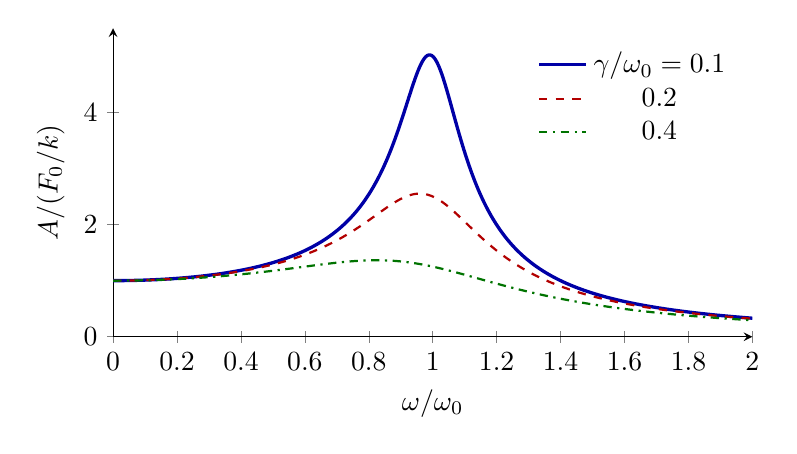
\begin{tikzpicture}
\begin{axis}[width=0.8\textwidth,height=5.5cm,axis lines=left,xlabel={$\omega/\omega_0$},ylabel={$A/(F_0/k)$},xmin=0,xmax=2,ymin=0,ymax=5.5,legend style={draw=none,at={(0.98,0.96)},anchor=north east},samples=400]
\addplot[blue!65!black,very thick,domain=0:2]{1/sqrt((1-x^2)^2+.04*x^2)};\addlegendentry{$\gamma/\omega_0=0.1$}
\addplot[red!70!black,thick,dashed,domain=0:2]{1/sqrt((1-x^2)^2+.16*x^2)};\addlegendentry{$0.2$}
\addplot[green!45!black,thick,dashdotted,domain=0:2]{1/sqrt((1-x^2)^2+.64*x^2)};\addlegendentry{$0.4$}
\end{axis}
\end{tikzpicture}
\caption{无量纲位移幅频曲线。图的纵轴由静态位移 $F_0/k$ 归一化；位移峰随阻尼偏移，不能直接拿它代替吸收功率峰。}
\label{fig:resonance-osc}
\end{figure}

\begin{example}[有限阻尼响应与无阻尼共振]
令驱动频率为 $\omega_0$。若 $\gamma>0$，稳态振幅为 $F_0/(2m\gamma\omega_0)$，相位滞后 $\pi/2$，并不随时间线性发散。若先令 $\gamma=0$，正弦和余弦已是齐次解，代回左端都给零。为产生与外力同相的余弦项，试取 $q_p=Ct\sin\omega_0t$。乘积求导给出 $\dot q_p=C(\sin\omega_0t+\omega_0t\cos\omega_0t)$，再求导并加上 $\omega_0^2q_p$，两个含 $t\sin\omega_0t$ 的项抵消：
\[
\ddot q_p+\omega_0^2q_p=2C\omega_0\cos\omega_0t,
\qquad C=\frac{F_0}{2m\omega_0}.
\]
零位移、零初速度下该特解就是全解。由此可见，先取长期稳态再令阻尼趋零，与先取无阻尼再观察有限时间，是不同极限。线性发散预告近似终会失效，不证明任何真实系统都按某种固定方式饱和。
\end{example}


\section{从精确方程到简正坐标}
两个摆连在一起时，轻推一只常会带动另一只。若能找到两只摆按固定比例一起动的方式，复杂运动就可以拆成几种简单振动。

\subsection{小参数如何进入}
把所有偏离平衡的量一起缩小，按它们缩小的快慢分组。保留决定首要恢复力和惯性的项，就会得到线性方程。

在本章自然系统的假设下，动能精确为
\begin{equation}
T=\frac12\sum_{a,b}M_{ab}(q)\dot q_a\dot q_b.
\label{eq:exact-T-multi}
\end{equation}
逐项求导得到
\[
\frac{\dd}{\dd t}T_{\dot q_a}=\sum_b M_{ab}\ddot q_b+
\sum_{b,c}M_{ab,q_c}\dot q_b\dot q_c,\qquad
T_{q_a}=\frac12\sum_{b,c}M_{bc,q_a}\dot q_b\dot q_c.
\]
把第二项对 $b,c$ 对称化，精确方程成为
\begin{equation}
\sum_bM_{ab}(q)\ddot q_b+
\sum_{b,c}\Gamma_{abc}(q)\dot q_b\dot q_c+V_{q_a}(q)=0,
\label{eq:exact-multi-eq}
\end{equation}
其中
\[
\Gamma_{abc}=\tfrac12(M_{ac,q_b}+M_{ab,q_c}-M_{bc,q_a}).
\]
$\Gamma$ 项来自坐标相关惯性，不是另加的外力。

令 $\eta=q-q_0$，定义 $M_0=M(q_0)$ 和精确余项
\begin{align*}
\mathcal N_a={}&-\sum_b[M_{ab}(q_0+\eta)-M_{ab}(q_0)]\ddot\eta_b\\
&-\sum_{b,c}\Gamma_{abc}(q_0+\eta)\dot\eta_b\dot\eta_c
-\left[V_{q_a}(q_0+\eta)-\sum_bK_{ab}\eta_b\right].
\end{align*}
于是 $M_0\ddot\eta+K\eta=\mathcal N$ 是精确重写。取固定长度、角度和时间尺度后，令 $\eta=\epsilon u$，并要求在考察的固定时间区间上 $u,\dot u,\ddot u$ 一致有界。三组余项分别是 $O(\epsilon^2)$、$O(\epsilon^2)$、$O(\epsilon^2)$，除以 $\epsilon$ 后均趋零。因此最低阶方程是
\begin{equation}
M_0\ddot{\boldsymbol\eta}+K\boldsymbol\eta=0,
\qquad
L_2=\tfrac12\dot{\boldsymbol\eta}^{\mathsf T}M_0\dot{\boldsymbol\eta}
-\tfrac12\boldsymbol\eta^{\mathsf T}K\boldsymbol\eta.
\label{eq:matrix-equation}
\end{equation}
也可直接在 $L$ 中数总阶次：$\eta\dot\eta^2$ 是三阶，$\dot\eta^2$ 是二阶。位移小而速度大不满足这一标度；小非线性频移在很长时间内还会积累相位差，不能把固定区间近似称为任意长时间精确。

\begin{physicsbox}
$M_0$ 是“移动这些坐标需要多少惯性”的二次型，$K$ 是“偏离平衡需要多少势能”的二次型。求频率要同时比较二者。弧度虽无量纲，摆角的惯性仍是转动惯量；把它误写为质点质量，会直接给出错误频率。
\end{physicsbox}

\subsection{广义本征值与质量加权}
假设各坐标以同一频率振动，振幅保持固定比例。代入后，刚度矩阵告诉我们恢复力，质量矩阵告诉我们各方向加速有多难。

以后简记 $M=M_0$。试解 $\eta=\bA e^{i\omega t}$，得到
\begin{equation}
K\bA=\lambda M\bA,\qquad \lambda=\omega^2,\qquad
\det(K-\lambda M)=0.
\label{eq:secular}
\end{equation}
行列式方程称为久期方程。有 $s$ 个实本征值（计重数），但它们为零或负时应分别求自由漂移或指数解，而非一律叫作实振动频率。

为何根一定实、能否总找齐振型？先把各坐标用固定尺度表示为数值，再取正定矩阵 $M$ 的对称正平方根。令
\[
y=M^{1/2}\eta,\qquad D=M^{-1/2}KM^{-1/2}=D^{\mathsf T}.
\]
因 $M$ 固定在平衡点，$\ddot\eta=M^{-1/2}\ddot y$。将它与 $\eta=M^{-1/2}y$ 代入，再左乘 $M^{-1/2}$，惯性项变成 $\ddot y$，故 $\ddot y+Dy=0$。实对称矩阵的谱定理给出正交矩阵 $O$，使
\[
O^{\mathsf T}DO=\Lambda=\operatorname{diag}(\lambda_1,\ldots,\lambda_s).
\]
取 $G=M^{-1/2}O$，则
\begin{equation}
G^{\mathsf T}MG=I,\quad G^{\mathsf T}KG=\Lambda,\quad
G^{-1}=G^{\mathsf T}M.
\label{eq:osc-simultaneous}
\end{equation}
例如 $G^{\mathsf T}MG=O^{\mathsf T}O=I$，而 $G^{\mathsf T}KG=O^{\mathsf T}DO=\Lambda$。第一式说明 $G^{\mathsf T}M$ 是 $G$ 的左逆，因 $G$ 是方阵，它也是逆矩阵。$DO=O\Lambda$ 左乘 $M^{1/2}$ 还给出 $KG=MG\Lambda$。于是 $G$ 的各列是完备、质量正交的振型。$M^{-1}K$ 通常不对称，不能直接把它交给只适用于实对称矩阵的数值程序。

设 $G$ 的第 $r$ 列为 $g_r$，定义质量归一化简正坐标
\begin{equation}
\eta=G\xi,\qquad \xi=G^{\mathsf T}M\eta.
\label{eq:normal-coordinates}
\end{equation}
代入二次型，得到
\[
T_2=\tfrac12\sum_r\dot\xi_r^2,\quad V_2=\tfrac12\sum_r\lambda_r\xi_r^2,
\qquad \ddot\xi_r+\lambda_r\xi_r=0.
\]
对 $\lambda_r=\omega_r^2>0$，初值解为
\begin{equation}
\xi_r(t)=(g_r^{\mathsf T}M\eta_i)\cos\omega_rt+
\frac{g_r^{\mathsf T}Mv_i}{\omega_r}\sin\omega_rt.
\label{eq:general-solution}
\end{equation}
$\lambda_r=0$ 时改为 $\xi_r(0)+\dot\xi_r(0)t$；$\lambda_r<0$ 时使用双曲正弦、余弦。若用未归一化振型 $a_r$ 展开 $\eta=\sum_r a_r c_r$，则
\[
c_r=\frac{a_r^{\mathsf T}M\eta}{a_r^{\mathsf T}Ma_r},\qquad
T_2=\frac12\sum_r(a_r^{\mathsf T}Ma_r)\dot c_r^2.
\]
这与质量归一化坐标的公式不同；改变振型长度会改变模态坐标的标度，物理位移保持不变。长度坐标下，$\xi$ 的单位一般为质量平方根乘长度。

\subsection{正交性、简并、坐标变换与频率估计}
若两种振动的频率不同，它们的正交性要按质量来衡量。频率相同则允许在同一个子空间里重选振型；用试探振型还能估计最低频率。

若 $Ka_r=\lambda_rMa_r$，利用对称性，有
\[
a_s^{\mathsf T}Ka_r=\lambda_r a_s^{\mathsf T}Ma_r
=\lambda_s a_s^{\mathsf T}Ma_r.
\]
故不同本征值的振型满足 $a_s^{\mathsf T}Ma_r=0$。重根时该等式本身不强迫正交，但谱定理允许在简并子空间内选质量正交基。重复频率不等于缺少振型；简并空间内的基旋转也不改变运动。

对非零试探方向 $a$，Rayleigh商为
\[
R(a)=\frac{a^{\mathsf T}Ka}{a^{\mathsf T}Ma}.
\]
把 $a=\sum_r b_rg_r$ 代入，得
\[
R(a)=\frac{\sum_r\lambda_rb_r^2}{\sum_r b_r^2},\qquad
\lambda_{\min}\le R(a)\le\lambda_{\max}.
\]
因此任一试探方向给最低本征值的上界，取遍方向才得到精确最小值；若有平移零模而只估计内部振动，必须先限制在其质量正交补。

换局部坐标 $\eta=Jz$，$J$ 可逆时，$M_z=J^{\mathsf T}MJ,K_z=J^{\mathsf T}KJ$，从而
\[
\det(K_z-\lambda M_z)=\det(J)^2\det(K-\lambda M).
\]
坐标单位或标度改变不改变频率。这也解释了为何只对 $K$ 做普通对角化通常不够。

\begin{keybox}
求解顺序：先核验平衡和坐标独立性，再求 $M,K$；检查对称性及 $M$ 正定；解广义本征值问题；按质量内积归一化；投影位置和速度初值；最后还原位移，并用原方程残差和能量核验。零模、负模和简并应在求根后分别处理。
\end{keybox}

\begin{modernbox}[title={进一步探索：陀螺项为什么另需处理}]
若二次拉格朗日量含 $\dot\eta^{\mathsf T}A\eta$，常矩阵 $A$ 的对称部分是全导数，反对称部分却给出
\[
M\ddot\eta+(A-A^{\mathsf T})\dot\eta+K\eta=0.
\]
令扰动按 $e^{i\omega t}$ 变化，得到频率方程 $\det[K-\omega^2M+i\omega(A-A^{\mathsf T})]=0$。第\ref{sec:sleeping-top}节给出含这种速度项的稳定例子。例如旋转参考系中的科里奥利项属于此类，不能只查 $K$ 的符号就套用前文判据。理解这一拓展需要第三章的速度耦合及复线性代数；本章核心仍限于无此项的自然系统。
\end{modernbox}


\section{耦合振动的典型模型}
以下几个模型都先回答三个问题。谁在动，谁把谁拉回去，怎样的集体动作能保持固定形状。

\subsection{双振子、耦合摆与拍}
把两只相同的摆同时往一边拉，或分别往相反方向拉，弹簧的伸长不同。只放开一只摆时，两种运动会叠在一起，并出现一快一慢的节奏。

\begin{example}[交叉项的符号决定哪个振型频率低]
设两个长度坐标的二次拉格朗日量为
\[
L_2=\frac m2(\dot x^2+\dot y^2)
-\frac{m\omega_0^2}{2}(x^2+y^2)+m\kappa xy,
\quad 0<\kappa<\omega_0^2.
\]
$\kappa$ 的单位为时间的负二次方。方程为
\[
\ddot x+\omega_0^2x-\kappa y=0,\qquad
\ddot y+\omega_0^2y-\kappa x=0.
\]
相加、相减分别得到
\[
\ddot c_++(\omega_0^2-\kappa)c_+=0,\quad
\ddot c_-+(\omega_0^2+\kappa)c_-=0,\quad
c_\pm=\frac{x\pm y}{\sqrt2}.
\]
故低频为同相 $(1,1)$，高频为反相 $(1,-1)$。直接代回两条原方程是最简单的符号检查。这里 $T_2=m(\dot c_+^2+\dot c_-^2)/2$；质量归一化坐标为 $\xi_\pm=\sqrt m\,c_\pm$。当 $\kappa=\omega_0^2$ 出现零模，超过该值势能有下降方向。
\end{example}

\begin{example}[无预紧耦合摆：先确定弹簧伸长]
两个固定支点等高，相距 $d>0$；两条轻刚杆长均为 $l$，摆锤质量均为 $m$。轻弹簧连接两摆锤，自然长度恰为 $d$、劲度 $k>0$。用同一向右为正的摆角 $\theta_1,\theta_2$，两端相对位置差为
\[
(d+l\sin\theta_2-l\sin\theta_1,\;l\cos\theta_1-l\cos\theta_2).
\]
弹簧长度减 $d$ 的一阶项为 $l(\theta_2-\theta_1)$，所以其二次势能是 $kl^2(\theta_2-\theta_1)^2/2$。这一步使用了无预紧假设；若弹簧已有张力，几何长度的二阶项也可能贡献刚度。
\[
M=ml^2I,\qquad
K=\begin{pmatrix}mgl+kl^2&-kl^2\\-kl^2&mgl+kl^2\end{pmatrix}.
\]
令 $d_\lambda=mgl+kl^2-ml^2\lambda$，久期式为 $(d_\lambda-kl^2)(d_\lambda+kl^2)=0$，得到
\begin{equation}
\omega_+^2=g/l,\quad a_+=(1,1)^{\mathsf T};\qquad
\omega_-^2=g/l+2k/m,\quad a_-=(1,-1)^{\mathsf T}.
\label{eq:coupled-pend-freq}
\end{equation}
同相运动中弹簧在该理想几何下长度不变；反相运动增加恢复力。两极限 $k\to0$ 给两个简并单摆，$g\to0$ 给整体横向零模与内部伸缩模。
\end{example}

\begin{figure}[htbp]
\centering
\begin{tikzpicture}[>=Stealth]
\foreach \shift/\sign/\lab in {0/1/同相低频,6/-1/反相高频}{
\begin{scope}[xshift=\shift cm]
\draw[thick](-.4,0)--(4,0);
\coordinate (P) at (0,0);\coordinate (Q) at (3,0);
\coordinate (B) at ({2*sin(12)},{-2*cos(12)});
\coordinate (C) at ({3+\sign*2*sin(12)},{-2*cos(12)});
\draw[dashed,gray](P)--(0,-2.2) (Q)--(3,-2.2);
\draw[blue!65!black,very thick](P)--(B) (Q)--(C);
\draw[green!45!black,thick,decorate,decoration={coil,aspect=.5,segment length=4pt,amplitude=3pt}](B)--(C);
\fill (P) circle(1.8pt);\fill (Q) circle(1.8pt);
\fill[blue!65!black](B)circle(3pt);\fill[blue!65!black](C)circle(3pt);
\draw[->,red!70!black,thick](0,-2.45)--(.65,-2.45);
\draw[->,red!70!black,thick](3,-2.45)--({3+\sign*.65},-2.45);
\node at (1.6,.35){\lab};
\end{scope}}
\end{tikzpicture}
\caption{耦合摆的两种振型快照。虚线为平衡位置，红箭头表示该快照的位移方向；弹簧严格连接两摆锤，而非连接平衡位置。左右图使用相同摆长和角度大小。}
\label{fig:coupled-pendulum}
\end{figure}

\begin{example}[只释放一只摆：从投影得到拍]
在上一模型中令 $\theta_1(0)=\Theta,\theta_2(0)=0$，初速度均为零。分解为两模各一半，得到
\begin{align*}
\theta_1&=\tfrac\Theta2(\cos\omega_+t+\cos\omega_-t)
=\Theta\cos(\bar\omega t)\cos(\Delta\omega t/2),\\
\theta_2&=\tfrac\Theta2(\cos\omega_+t-\cos\omega_-t)
=\Theta\sin(\bar\omega t)\sin(\Delta\omega t/2),
\end{align*}
其中 $\bar\omega=(\omega_-+\omega_+)/2$、$\Delta\omega=\omega_--\omega_+>0$。弱耦合 $k/m\ll g/l$ 时，快振动由慢包络调制，第一次近乎完全转移发生在 $t\simeq\pi/\Delta\omega$。取 $k/m=0.1g/l$，则 $\omega_-/\omega_+=\sqrt{1.2}$，首次转移约在 $\omega_+t=32.9$。

每个简正模的能量恒定。说“能量在两摆间交换”时，局部能量怎样分配耦合弹簧有约定；弱耦合下，分别用两只裸单摆的能量观察交换最直观。$k\to0$ 时差频趋零，转移时间发散，不发生无耦合能量传递。
\end{example}

\begin{figure}[htbp]
\centering
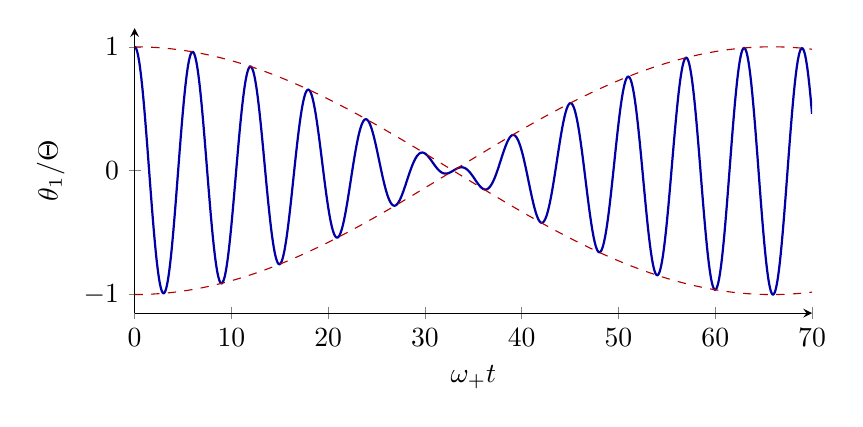
\begin{tikzpicture}
\begin{axis}[width=.84\textwidth,height=5.2cm,xlabel={$\omega_+t$},ylabel={$\theta_1/\Theta$},xmin=0,xmax=70,ymin=-1.15,ymax=1.15,axis lines=left,samples=1000]
\addplot[blue!65!black,thick,domain=0:70]{.5*(cos(deg(x))+cos(deg(sqrt(1.2)*x)))};
\addplot[red!70!black,dashed,domain=0:70]{cos(deg((sqrt(1.2)-1)*x/2))};
\addplot[red!70!black,dashed,domain=0:70]{-cos(deg((sqrt(1.2)-1)*x/2))};
\end{axis}
\end{tikzpicture}
\caption{耦合摆的拍：蓝线严格取正文的线性叠加解，红虚线为其有符号包络的正负两支。包络消失并不代表两个简正模的能量消失。}
\label{fig:osc-beats}
\end{figure}

\subsection{不等质量与双摆}
两只质量不同时，同样的位移并不意味着同样的惯性。双摆还要注意，下球速度受到两根杆的转动共同影响。

\begin{example}[欧氏不正交，质量内积仍正交]
两质点质量为 $m,2m$，左端与墙连接劲度 $k$ 的弹簧，两质点间连接劲度 $2k$ 的弹簧，第二质点与右墙也连接劲度 $2k$ 的弹簧。沿直线的平衡位移为 $x_1,x_2$，质量矩阵为 $M=m\operatorname{diag}(1,2)$，刚度矩阵为
\[
K=k\begin{pmatrix}3&-2\\-2&4\end{pmatrix}.
\]
记 $z=m\lambda/k$，久期式为
\[
(3-z)(4-2z)-4=2(z-1)(z-4)=0.
\]
故 $\omega_1^2=k/m,\omega_2^2=4k/m$，未归一化振型为 $(1,1)$ 与 $(2,-1)$。其普通点积为1，而
\[
(1,1)M(2,-1)^{\mathsf T}=0.
\]
质量归一化矩阵及投影为
\begin{equation}
G=\left(\frac{(1,1)^{\mathsf T}}{\sqrt{3m}},
\frac{(2,-1)^{\mathsf T}}{\sqrt{6m}}\right),\quad
\xi_1=\sqrt{\frac m3}(x_1+2x_2),\quad
\xi_2=\sqrt{\frac{2m}3}(x_1-x_2).
\label{eq:osc-unequal-G}
\end{equation}
代回验证 $G^{\mathsf T}MG=I$、$G^{\mathsf T}KG=\operatorname{diag}(k/m,4k/m)$。若 $x(0)=(a,0),\dot x(0)=0$，
\[
x(t)=\frac a3(1,1)^{\mathsf T}\cos\sqrt{k/m}\,t
+\frac a3(2,-1)^{\mathsf T}\cos(2\sqrt{k/m}\,t).
\]
初始总能量为 $3ka^2/2$，两模能量分别为 $ka^2/6$ 与 $4ka^2/3$，相加一致。
\end{example}

\begin{example}[双摆：同样两根杆，惯性有交叉项]
在式 \eqref{eq:lag-double-pendulum} 中取 $m_1=m_2=m,\ l_1=l_2=l$，两角都从向下竖直量起，在 $(0,0)$ 附近线性化。
沿用第三章的两个绝对摆角，取 $m_1=m_2=m,l_1=l_2=l$，在最低平衡展开。二次型为
\[
T_2=\tfrac12ml^2(2\dot\theta_1^2+2\dot\theta_1\dot\theta_2+\dot\theta_2^2),\quad
V_2=\tfrac12mgl(2\theta_1^2+\theta_2^2).
\]
这里两杆之间没有弹簧，耦合来自下球速度包含上球运动。
\[
M=ml^2\begin{pmatrix}2&1\\1&1\end{pmatrix},\quad
K=mgl\begin{pmatrix}2&0\\0&1\end{pmatrix}.
\]
令 $z=\omega^2l/g$，行列式给出
\[
(2-2z)(1-z)-z^2=z^2-4z+2=0.
\]
因此
\begin{equation}
\omega_{\rm low}^2=(2-\sqrt2)g/l,\quad a_{\rm low}=(1,\sqrt2)^{\mathsf T};\qquad
\omega_{\rm high}^2=(2+\sqrt2)g/l,\quad a_{\rm high}=(1,-\sqrt2)^{\mathsf T}.
\label{eq:osc-double-pend}
\end{equation}
以第一行求角度比 $a_2/a_1=2(1-z)/z$，即可独立检查正负。两振型质量范数平方为 $ml^2(4\pm2\sqrt2)$，且彼此质量正交。给定小角初值后应按式 \eqref{eq:general-solution} 投影，不能各自用单摆频率 $\sqrt{g/l}$。
\end{example}

\begin{figure}[htbp]
\centering
\begin{tikzpicture}[>=Stealth]
\foreach \shift/\sgn/\lab in {0/1/低频同向,5.8/-1/高频反向}{
\begin{scope}[xshift=\shift cm]
\coordinate(O)at(0,0);
\coordinate(A)at({2*sin(8)},{-2*cos(8)});
\coordinate(B)at({2*sin(8)+2*sin(\sgn*sqrt(2)*8)},{-2*cos(8)-2*cos(\sgn*sqrt(2)*8)});
\draw[dashed,gray](O)--(0,-4.2);
\draw[dashed,gray](A)--++(0,-2.1);
\draw[very thick,blue!65!black](O)--(A)--(B);
\fill(O)circle(2pt);\fill(A)circle(3pt)node[right]{$m$};\fill(B)circle(3pt)node[right]{$m$};
\draw[->,red!70!black](0,-1.8)--(.55,-1.8);
\draw[->,red!70!black](0,-4.4)--({.55*(1+\sgn*sqrt(2))},-4.4);
\node at (.3,.4){\lab};
\end{scope}}
\end{tikzpicture}
\caption{双摆两振型，取 $\theta_1=8^\circ,\theta_2=\pm\sqrt2\theta_1$ 画几何快照。红箭头表示质点横向位移的线性近似：第二球位移是 $l(\theta_1+\theta_2)$，不只由第二杆角度决定。}
\label{fig:osc-double-modes}
\end{figure}

\subsection{纵向三原子模型与零模}
把三颗质点一起平移，各段弹簧的长度都不变。剩下的两种独立动作才会伸缩弹簧并产生恢复力。

\begin{example}[伸缩频率与质心分离]
三个质点沿轴运动，质量为 $m,\mu,m$，两条相同轻弹簧劲度为 $k$，用 $x_i$ 表示相对平衡的轴向位移。模型只保留纵向自由度：
\[
M=\operatorname{diag}(m,\mu,m),\quad
V_2=\tfrac k2(x_2-x_1)^2+\tfrac k2(x_3-x_2)^2,\quad
K=k\begin{pmatrix}1&-1&0\\-1&2&-1\\0&-1&1\end{pmatrix}.
\]
先直接作用于 $(1,1,1)$，得零本征值。其坐标是质心平移，$X_{\rm cm}=(mx_1+\mu x_2+mx_3)/(2m+\mu)$ 满足 $\ddot X_{\rm cm}=0$。

取端点反向 $a_1=(1,0,-1)$，有 $Ka_1=(k/m)Ma_1$，故 $\omega_1^2=k/m$。再取端点同向 $(1,b,1)$，非零模必须与平移模质量正交，因而 $2m+\mu b=0$，$b=-2m/\mu$。第一行方程给出
\[
\omega_2^2=\frac{k}{m}(1-b)=k\left(\frac1m+\frac2\mu\right),\qquad
 a_2=(1,-2m/\mu,1).
\]
三组范数平方分别为 $2m+\mu,2m,2m+4m^2/\mu$，除以各自范数就得到 $G$。每个非零模满足总动量为零；例如 $\mu\to\infty$ 时中心近乎固定，两伸缩频率趋于简并。

为防止“同相”命名歧义，直接看两段键长变化 $\delta d_1=x_2-x_1,\delta d_2=x_3-x_2$：第一伸缩模两段同时伸长/缩短，是对称伸缩；第二伸缩模一长一短，是反对称伸缩。原子位移的对称性还须考虑空间反演使矢量反向。
\end{example}

\begin{figure}[htbp]
\centering
\begin{tikzpicture}[>=Stealth]
\foreach \yy/\sgn/\lab in {0/-1/两键同伸缩,-2.2/1/两键反向伸缩}{
\node[anchor=east]at(-.7,\yy){\lab};
\foreach \xx/\mass in {0/m,2/\mu,4/m}{\draw[fill=blue!10](\xx,\yy)circle(.19);\node[below]at(\xx,\yy-.25){$\mass$};}
\draw[decorate,decoration={coil,aspect=.5,segment length=4pt,amplitude=3pt},green!45!black,thick](.19,\yy)--(1.81,\yy) (2.19,\yy)--(3.81,\yy);
\draw[red!70!black,->,thick](0,\yy+.5)--(.6,\yy+.5);
\draw[red!70!black,->,thick](4,\yy+.5)--({4+\sgn*.6},\yy+.5);
}
\node at(2,.52){$0$};
\draw[red!70!black,->,thick](2,-1.7)--(.8,-1.7);
\end{tikzpicture}
\caption{三质点模型的两个伸缩模，箭头表示位移振幅。本图取 $\mu=m$，下排幅度比严格为 $1:-2:1$；上排为 $1:0:-1$。整体平移零模未画。}
\label{fig:triatomic}
\end{figure}

\begin{modernbox}[title={进一步探索：从振型到光谱还缺什么？}]
这个模型说明质量、刚度与伸缩频率的关系；同位素改变质量而近似保留势能曲率，是应用广义本征值的一个切入点。但真实分子还有横向、转动自由度和电子结构。一个模能否被红外或拉曼观测到，还分别取决于偶极矩或极化率随该模是否变化，不能把所有数学振型都说成吸收峰。继续学习需三维振动、对称性及电磁耦合；本例不拟合具体分子的实验谱线。
\end{modernbox}


\section{模态受迫响应与阻尼的限制}
外力若顺着某个振型推，通常更容易把这个模激发出来。阻尼器若只装在一个位置，则可能同时感受到几个模的速度。

\subsection{广义力如何激发某个模}
把外力在各振型上的分量算出来，就能判断直接推到了哪些模。若模态阻尼矩阵有非对角项，一个模还可能被另一个模带动。

若有小外力向量 $f(t)$ 和线性黏性矩阵 $C=C^{\mathsf T}\ge0$，则
\begin{equation}
M\ddot\eta+C\dot\eta+K\eta=f(t),\qquad
\dot E_2=\dot\eta^{\mathsf T}f-\dot\eta^{\mathsf T}C\dot\eta.
\label{eq:osc-multi-driven}
\end{equation}
采用无阻尼振型 $\eta=G\xi$ 并左乘 $G^{\mathsf T}$，得到
\[
\ddot\xi+C_N\dot\xi+\Lambda\xi=f_N(t),\qquad
C_N=G^{\mathsf T}CG,\quad f_N=G^{\mathsf T}f.
\]
模态力 $f_{N,r}=g_r^{\mathsf T}f$ 不是 $g_r^{\mathsf T}Mf$；质量已经在惯性归一化中处理。对 $\Lambda>0$ 且 $C_N$ 为对角阵的情形，每个模有独立响应
\[
\xi_r^{\rm st}=\operatorname{Re}\left[
\frac{g_r^{\mathsf T}F}{\omega_r^2-\omega^2+i c_r\omega}e^{i\omega t}\right],\qquad
c_r=(C_N)_{rr}.
\]
若模态力为零，即使驱动频率靠近该本征频率，也不激发这个模。阻尼为零时，该式只适用于非共振特解，并不意味着初始自由响应会消失。

一个常用而受限的选择是比例阻尼 $C=\alpha M+\beta K$，此时
\[
C_N=\alpha I+\beta\Lambda,\quad c_r=\alpha+\beta\omega_r^2,
\]
$\alpha$ 的单位为时间的负一次方，$\beta$ 为时间。只要求模型总 $C$ 半正定；$\alpha,\beta\ge0$ 是保证它的一种充分选择。

\begin{example}[一个局部阻尼器一般耦合无阻尼模]
取式 \eqref{eq:osc-unequal-G} 的两质量模型，只在第一质点与墙之间加阻尼器，$C=\operatorname{diag}(c,0)$。则
\[
C_N=\frac c m\begin{pmatrix}1/3&\sqrt2/3\\\sqrt2/3&2/3\end{pmatrix}.
\]
非对角元不为零，两个无阻尼简正坐标通过速度耦合。尽管 $\dot E_2=-c\dot x_1^2\le0$，不能分别往两个独立简谐方程随意加衰减率；弱阻尼下忽略非对角项也需额外论证。一般谐波响应应直接解
\[
(K-\omega^2M+i\omega C)X=F.
\]
能量不增本身不保证任一模型的所有模都会衰减到零；可能存在阻尼看不到的运动方向。

因为阻尼只作用于第一坐标，变换后有 $(C_N)_{rs}=c(g_r)_1(g_s)_1$。第一行的两个振型分量是 $1/\sqrt{3m}$、$2/\sqrt{6m}$，所以交叉元为 $\sqrt2c/(3m)$。这也可从耗散功率 $-c[(g_1)_1\dot\xi_1+(g_2)_1\dot\xi_2]^2$ 的交叉项核对。
\end{example}

\begin{example}[调谐吸振器：共振之外还有反共振]
主质量 $m$ 由劲度 $k$ 的弹簧连墙，附加质量 $\mu$ 通过劲度 $\kappa$ 的弹簧连主质量，均沿直线无摩擦运动。对主质量施加 $F_0\cos\omega t$，两个平衡位移为 $x_1,x_2$，有
\[
M=\begin{pmatrix}m&0\\0&\mu\end{pmatrix},\quad
K=\begin{pmatrix}k+\kappa&-\kappa\\-\kappa&\kappa\end{pmatrix},\quad
F=(F_0,0)^{\mathsf T}.
\]
无阻尼、避开本征频率时，解两条代数方程得
\begin{align*}
X_1&=\frac{(\kappa-\mu\omega^2)F_0}{D(\omega)},\quad
X_2=\frac{\kappa F_0}{D(\omega)},\\
D(\omega)&=(k+\kappa-m\omega^2)(\kappa-\mu\omega^2)-\kappa^2.
\end{align*}
当 $\omega_a^2=\kappa/\mu$ 时，$D=-\kappa^2\ne0$，因此
\[
X_1=0,\qquad X_2=-F_0/\kappa.
\]
附加弹簧力恰好抵消驱动，主质量的受迫分量为零，这是反共振，不是整个系统没有运动。取调谐条件 $\kappa/\mu=k/m$，即可在原主振子频率消除理想特解的主质量位移；两个新本征频率则由 $D=0$ 给出。

该结论针对指定频率的无阻尼特解。任意初值会叠加不衰减的自由振动；阻尼、失谐和有限行程也会改变零点附近响应。因此不能据此宣称任意扰动或任意频率都被消除。
\end{example}

\begin{figure}[htbp]
\centering
\begin{tikzpicture}[>=Stealth]
\draw[thick](-.2,-.5)--(-.2,.7);
\draw[decorate,decoration={coil,aspect=.5,segment length=5pt,amplitude=4pt},thick](-.2,.1)--(1.6,.1)node[midway,above=.18cm]{$k$};
\draw[fill=blue!10](1.6,-.35)rectangle(2.7,.55);\node at(2.15,.1){$m$};
\draw[decorate,decoration={coil,aspect=.5,segment length=5pt,amplitude=4pt},thick](2.7,.1)--(4.7,.1)node[midway,above=.18cm]{$\kappa$};
\draw[fill=green!10](4.7,-.35)rectangle(5.6,.55);\node at(5.15,.1){$\mu$};
\draw[->,red!70!black,thick](2.15,.9)--(3.6,.9)node[right]{$F_0\cos\omega t$};
\draw[->](1.8,-.7)--(2.8,-.7)node[right]{$x_1$};\draw[->](4.7,-.7)--(5.7,-.7)node[right]{$x_2$};
\end{tikzpicture}
\caption{理想调谐吸振器。附加质量的运动产生补偿主驱动的弹簧力；主质量反共振频率与两自由度系统的本征频率不同。}
\label{fig:osc-absorber}
\end{figure}


\section{从有限链到长波连续极限}
许多质点排成一列时，一个质点的运动可沿弹簧传给邻居。先看一串有限质点允许哪些波，再看波长远大于间距时如何近似为连续介质。

\subsection{周期边界、色散与模态计数}
把链的两端接成环，绕一圈后的位移必须接得上。这个要求使波数只能取离散值；固定两端时则要满足另一套条件。

把 $N\ge3$ 个质量为 $m$ 的质点放在一维周期单元中，相邻间隔为 $a$，纵向位移为 $u_n$，周期边界 $u_{n+N}=u_n$。这里只把周期边界当作理想无限链的有限近似，不引入实际圆环弯曲的几何力。相邻弹簧劲度均为 $k$，则
\begin{equation}
m\ddot u_n=k(u_{n+1}+u_{n-1}-2u_n).
\label{eq:chain-eq}
\end{equation}
试解 $u_n=Ae^{i(pna-\omega t)}$，周期边界要求 $p=2\pi j/(Na)$，$j$ 为整数。代入并消去公共因子，得到
\[
-m\omega^2=k(e^{ipa}+e^{-ipa}-2)=-4k\sin^2(pa/2),
\]
所以
\begin{equation}
\omega(p)=2\sqrt{k/m}\,|\sin(pa/2)|.
\label{eq:dispersion-chain}
\end{equation}
$p$ 与 $p+2\pi/a$ 在所有格点给同一位形，因此取第一布里渊区 $-\pi<pa\le\pi$ 就足够；并非区外完全没有数学表示。$p=0$ 是整体平移零模。

对 $0<pa<\pi$，$\pm p$ 是同频的复共轭对，实基可选 $\cos pna$ 与 $\sin pna$。它们合起来只有两个实位形自由度，不能把共轭波数再各算两个。若 $N$ 偶数，$pa=\pi$ 的格点正弦恒零，只剩一个交替位移模；这加上零模和其余波数对，恰给 $N$ 个实坐标。

\begin{figure}[htbp]
\centering
\begin{tikzpicture}
\begin{axis}[width=.82\textwidth,height=5.3cm,axis lines=left,xlabel={$pa/\pi$},ylabel={$\omega/\sqrt{k/m}$},xmin=-1.05,xmax=1.05,ymin=0,ymax=3.4,legend style={at={(.5,.98)},anchor=north,draw=none,font=\small},samples=240]
\addplot[blue!65!black,very thick,domain=-1:1]{2*abs(sin(deg(pi*x/2)))};\addlegendentry{离散链}
\addplot[red!70!black,dashed,domain=-1:1]{pi*abs(x)};\addlegendentry{长波近似}
\addplot[only marks,mark=*,mark size=1.7pt,blue!65!black]coordinates{(-.75,1.847759)(-.5,1.414214)(-.25,.765367)(0,0)(.25,.765367)(.5,1.414214)(.75,1.847759)(1,2)};
\end{axis}
\end{tikzpicture}
\caption{第一布里渊区内的准确色散与 $\omega\simeq a\sqrt{k/m}|p|$。在当前横轴下，长波直线斜率为 $\pi$；圆点为 $N=8$ 周期链的允许波数，$-\pi$ 与 $\pi$ 是同一格点模。}
\label{fig:dispersion}
\end{figure}

\subsection{相速度、群速度与边界}
波峰移动的速度和一群相近波叠成的包络速度可以不同。看清题目追踪的是波峰还是包络，再选相速度或群速度。

对正波数，定义
\[
v_{\rm ph}=\omega/p,\qquad
v_g=\frac{\dd\omega}{\dd p}=a\sqrt{k/m}\cos(pa/2).
\]
群速度描述在无限或足够长的无耗散链中，窄波数包络的传播；有限环会有回返，单个驻波也没有可以追踪的行进包络。长波 $|pa|\ll1$ 时两速度均趋 $c_s=a\sqrt{k/m}$；区边界相邻格点反相、$v_g=0$，但 $\omega=2\sqrt{k/m}$ 并不为零。

\begin{example}[固定端与周期端不可混用]
另取 $N$ 个活动质点，左右固定端 $u_0=u_{N+1}=0$。令振型为 $u_n=A\sin(pna)$，边界给
\[
p_j a=\frac{j\pi}{N+1},\quad
\omega_j=2\sqrt{k/m}\sin\frac{j\pi}{2(N+1)},\quad j=1,\ldots,N.
\]
全部频率正，无整体平移模。最小频率在大 $N$ 时约为 $\pi c_s/[(N+1)a]$。同样的局部弹簧方程，不同边界改变允许波数和模态形状；不能只记色散式而丢掉边界条件。
\end{example}

\subsection{长波展开与连续能量}
波长远大于质点间距时，相邻两点的位移差可用斜率乘间距近似。把每一小段的质量和弹性加起来，就得到连续模型。

用平滑场 $u(x,t)$ 插值格点，$x=na$，泰勒展开使奇数空间导数相消：
\[
u(x+a)+u(x-a)-2u(x)
=a^2u_{xx}+\frac{a^4}{12}u_{xxxx}+\cdots.
\]
保留最低阶得
\begin{equation}
u_{tt}=c_s^2u_{xx},\qquad c_s^2=ka^2/m.
\label{eq:wave-equation}
\end{equation}
忽略项相对大小约为 $(pa)^2/12$。这个近似只用于长波，不能把截断高阶方程任意外推到区边界。

连续质量密度 $\rho=m/a$，纵向弹性系数 $\mathcal C=ka$，离散能量相应趋于
\[
T\simeq\frac12\int\rho u_t^2\,\dd x,\qquad
V\simeq\frac12\int\mathcal C u_x^2\,\dd x,\qquad
c_s^2=\mathcal C/\rho.
\]
变分给出波动方程，同时边界项为 $\mathcal C u_x\delta u$：固定端取 $\delta u=0$，自由端取 $\mathcal C u_x=0$。本例是纵向弹性链，不能把 $k$ 直接当作弦张力。若真的取 $a\to0$ 且保持有限连续介质，须按 $m=\rho a,k=\mathcal C/a$ 缩放；固定 $m,k$ 而只令 $a\to0$ 会使声速趋零。

\begin{modernbox}[title={进一步探索：声子与有限模态}]
每个正频简正坐标都是谐振子。若进一步量子化，其能级为 $E_n=\hbar\omega(n+1/2)$，振动量子称为声子；这里需要量子谐振子基础。零频整体平移不能照搬这一束缚振子能级式。色散给频率与波数关系，但有限温度热输运还需模占据、边界及散射，不是由本章无耗散链单独决定。
\end{modernbox}


\section{进一步探索：线性理论之外}
位移增大或外部机构开始周期地改变刚度时，线性定常模型会漏掉一些现象。下面用几个简单模型看看最早出现的修正。

本节不把弱非线性结果混入前文的精确线性叠加。它回答两个问题：被略去的项首先改变什么？周期改变参数为何不同于施加外力？

\subsection{幅频移动与组合频率}
理想弹簧振得大些和小些，周期相同。加入更高次恢复力后，周期可能随振幅变化，几个模一起运动时也可能产生新的组合频率。

\begin{example}[对称四次势能的首阶频移]
取
\[
V(q)=\tfrac12m\omega_0^2q^2+\tfrac14\beta q^4,\qquad
\ddot q+\omega_0^2q+\frac\beta m q^3=0.
\]
$\beta$ 在势能和方程中的含义保持一致。令转折振幅为 $A$，小参数为 $|\beta|A^2/(m\omega_0^2)\ll1$。最低阶取 $q=A\cos\omega t$，用 $\cos^3z=(3\cos z+\cos3z)/4$，基频项系数为
\[
A\left[-\omega^2+\omega_0^2+\frac{3\beta A^2}{4m}\right].
\]
消除这一阶的基频残差，得到
\begin{equation}
\omega=\omega_0+\frac{3\beta A^2}{8m\omega_0}
+O\left(\omega_0\left[\frac{\beta A^2}{m\omega_0^2}\right]^2\right).
\label{eq:osc-duffing-shift}
\end{equation}
还存在小三次谐波，不能说解仍是精确正弦。$\beta>0$ 为硬化，$\beta<0$ 为局部软化；负四次项在大位移不提供全局束缚，本近似只在原点附近小能量势阱内使用。若势能另有三次项，其二阶效应也可贡献频移，不能照搬这个对称势公式。
\end{example}

\begin{example}[从明确的耦合势产生和频、差频]
取三个等效质量 $m$ 的坐标，势能含 $\epsilon c q_1q_2q_3$，$c$ 的单位使该项为能量；$\epsilon$ 为无量纲小参数。在有限时间的最低阶，令
\[
q_1^{(0)}=A\cos\omega_1t,\qquad q_2^{(0)}=B\cos\omega_2t,
\]
则第三模的一阶受迫式含
\[
\ddot q_3+\omega_3^2q_3
=-\frac{\epsilon c AB}{2m}
[\cos(\omega_1+\omega_2)t+\cos(\omega_1-\omega_2)t].
\]
非共振时，一个频率 $\nu$ 的力 $f\cos\nu t$ 给特解 $f\cos\nu t/(\omega_3^2-\nu^2)$；若 $\nu=\omega_3$，首阶特解为 $ft\sin\omega_3t/(2\omega_3)$。这表示普通展开将出现长期失效，须跟踪各模振幅反馈，不能把线性增长当成封闭非线性系统的无限能量来源。此三次势也只作为局部模型，远处可需高阶稳定项。
\end{example}

\subsection{主参数共振的慢变振幅推导}
荡秋千时按时改变身体姿势，等于周期地改变系统参数。这里先找调制节拍与自由振动的关系，再看输入能量能否抵消阻尼。

\begin{example}[刚度调制如何克服阻尼]
取
\begin{equation}
\ddot q+2\gamma\dot q+\omega_0^2[1+\epsilon\cos\Omega t]q=0,
\quad 0<\epsilon\ll1,\quad
\delta=\Omega-2\omega_0=O(\epsilon\omega_0),\quad
\gamma=O(\epsilon\omega_0).
\label{eq:mathieu}
\end{equation}
当 $\gamma=0$ 时，这是马蒂厄方程的一种参数化。取试探振荡的载波角频率 $\omega_{\rm c}=\Omega/2$，
\[
q=a(t)\cos\omega_{\rm c} t+b(t)\sin\omega_{\rm c} t,
\]
$a,b$ 在一个振动周期内只作 $O(\epsilon)$ 的相对尺度变化。一阶计算中，$\ddot q+\omega_{\rm c}^2q$ 的慢项是 $2\omega_{\rm c}(\dot b\cos\omega_{\rm c} t-\dot a\sin\omega_{\rm c} t)$，含 $\ddot a,\ddot b$ 的项为二阶。阻尼只需乘 $\dot q$ 的快项，因为 $\gamma\dot a,\gamma\dot b$ 也是二阶。调制项用
\[
\cos2\omega_{\rm c} t\,\cos\omega_{\rm c} t=\tfrac12(\cos3\omega_{\rm c} t+\cos\omega_{\rm c} t),\quad
\cos2\omega_{\rm c} t\,\sin\omega_{\rm c} t=\tfrac12(\sin3\omega_{\rm c} t-\sin\omega_{\rm c} t).
\]
在一周期投影到 $\cos\omega_{\rm c} t,\sin\omega_{\rm c} t$ 时，$3\omega_{\rm c}$ 项与二者正交。两条投影方程为
\begin{align*}
2\omega_{\rm c}\dot b+2\gamma\omega_{\rm c} b+(\omega_0^2-\omega_{\rm c}^2+\epsilon\omega_0^2/2)a&=0,\\
-2\omega_{\rm c}\dot a-2\gamma\omega_{\rm c} a+(\omega_0^2-\omega_{\rm c}^2-\epsilon\omega_0^2/2)b&=0.
\end{align*}
因为 $\omega_{\rm c}=\omega_0+\delta/2$，有 $(\omega_0^2-\omega_{\rm c}^2)/(2\omega_{\rm c})=-\delta/2+O(\epsilon^2\omega_0)$。调制项的系数 $\epsilon\omega_0^2/(4\omega_{\rm c})$ 可在同一精度下取 $\epsilon\omega_0/4$。记 $h=\epsilon\omega_0/4$，化成
\[
\frac{\dd}{\dd t}\begin{pmatrix}a\\b\end{pmatrix}
=\begin{pmatrix}-\gamma&-\delta/2-h\\\delta/2-h&-\gamma\end{pmatrix}
\begin{pmatrix}a\\b\end{pmatrix}.
\]
设慢振幅与 $e^{st}$ 成正比。系数矩阵减去 $sI$ 后的行列式为 $(s+\gamma)^2-(h^2-\delta^2/4)$，令它为零得两个慢指数
\begin{equation}
s_\pm=-\gamma\pm\sqrt{h^2-\delta^2/4}.
\label{eq:osc-param-growth}
\end{equation}
因此无阻尼主不稳定区在首阶为 $|\delta|<\epsilon\omega_0/2$。有阻尼时需 $h^2>\gamma^2+\delta^2/4$；正调谐 $\delta=0$ 的阈值为 $\epsilon>4\gamma/\omega_0$。边界附近高阶修正会影响判断，这不是任意调制深度下的精确稳定图。

调制中的瞬时机械能取
\[
E(t)=\tfrac m2\dot q^2+\tfrac{m\omega_0^2}2[1+\epsilon\cos\Omega t]q^2,
\quad
\dot E=-2m\gamma\dot q^2-\frac{m\omega_0^2\epsilon\Omega}{2}\sin\Omega t\,q^2.
\]
第二项是改变刚度的机构输入/取出的功率。$q\equiv0$ 仍为精确解；“不稳定”表示存在增长的微扰，不表示零初态自行产生非零运动，也不是每个特选初值都会增长。
\end{example}

\begin{figure}[htbp]
\centering
\begin{tikzpicture}
\begin{axis}[width=.78\textwidth,height=5.2cm,axis lines=left,xlabel={$\Omega/\omega_0$},ylabel={$\epsilon$},xmin=1.8,xmax=2.2,ymin=0,ymax=.32,xtick={1.8,1.9,2,2.1,2.2},ytick={0,.1,.2,.3}]
\fill[red!12](axis cs:2,0)--(axis cs:1.85,.3)--(axis cs:2.15,.3)--cycle;
\addplot[red!70!black,thick,domain=0:.3]({2-x/2},x);
\addplot[red!70!black,thick,domain=0:.3]({2+x/2},x);
\node at(axis cs:2,.23){首阶不稳定区};
\end{axis}
\end{tikzpicture}
\caption{无阻尼、弱调制的主舌形区首阶边界 $\Omega/\omega_0=2\pm\epsilon/2$。舌尖在零调制处收拢，宽度随调制增大；本图不画高阶窄舌，也不冒充完整精确的马蒂厄稳定图。}
\label{fig:parametric}
\end{figure}

周期系数问题可用弗洛凯（Floquet）方法。取状态 $(q,\dot q)^{\mathsf T}$，分别以 $(1,0)^{\mathsf T}$、$(0,1)^{\mathsf T}$ 为初值，推进一个调制周期 $T_{\rm m}=2\pi/\Omega$。将所得两列并排，得到单周期矩阵 $U$。系数每周期复原，所以第 $n$ 个周期末的状态由 $U^n$ 给出，$U$ 的本征值称为弗洛凯乘子。若某乘子模大于1，相应模随周期数指数增长。无阻尼时，两个解的行列式 $W=q_1\dot q_2-\dot q_1q_2$ 满足 $\dot W=q_1\ddot q_2-\ddot q_1q_2=0$，故 $\det U=1$。若模为1的重根只有一个本征方向，$U^n$ 中还会出现正比于 $n$ 的项。NIST的马蒂厄稳定图使用标准参数 $(a,q)$，若要比较，先作 $z=\Omega t/2$，得到
\[
\frac{\dd^2q_{\rm osc}}{\dd z^2}+[a-2q_{\rm M}\cos2z]q_{\rm osc}=0,\quad
a=\frac{4\omega_0^2}{\Omega^2},\quad q_{\rm M}=-\frac{2\epsilon\omega_0^2}{\Omega^2}.
\]
这里 $q_{\rm osc}$ 是位移，$q_{\rm M}$ 是马蒂厄参数，二者不同；这一映射限于无阻尼式。

\subsection{自激、分岔与混沌：不由二次型包办}
外力一直按节拍推、系统自己补充振动能量、以及初值很接近却逐渐分离，是不同的现象。下面用不同的判据来区分。

范德波尔模型可写成无量纲形式
\[
x''-\mu(1-x^2)x'+x=0,\quad \mu>0,
\]
撇号表示对无量纲时间求导，$x$ 也无量纲。能量 $e=(x'^2+x^2)/2$ 满足 $e'=\mu(1-x^2)x'^2$，小位移区可注入能量，大位移区可耗散。弱 $\mu$ 下令 $x\simeq A\cos(\tau+\phi)$，用
\[
\overline{x'^2}=A^2/2,\quad \overline{x^2x'^2}=A^4/8,
\]
得到 $A'=\mu A(1-A^2/4)/2$。$A=2$ 是这一平均方程的稳定振幅，不是任意 $\mu$ 下精确正弦轨道；相位还与初始条件有关。原点精确初态仍停在原点，极限环也不是保守系统的能量等高线。

分岔研究的是改变参数后解的结构如何改变。例如 $V(q)=rq^2/2+bq^4/4$、$b>0$，平衡为 $q=0$ 及 $r<0$ 时的 $q=\pm\sqrt{-r/b}$；$r=0$ 处二次曲率消失，必须保留四次项。混沌则需更丰富的动力学，不能从单个频移、拍或短时轨道分离就断定；二维光滑自治范德波尔系统的平面极限环也不等于混沌。进一步研究需非线性方程、相空间与稳定性理论，超出本章简正模求解。

\section{计算与模拟：用残差和收敛检验模型}
把求出的振型代回原方程，检查两边差多少。再分别缩小初始振幅和积分步长，区分小角近似误差与计算误差。

伴随脚本 \texttt{review/verify\_ch04.py} 使用标准Python库，结果保存在
\begin{center}\texttt{ch04\_verification\_results.json}\end{center}
主要检查包括：
\begin{enumerate}[leftmargin=1.8em]
\item 对每个解析振型计算 $Ka_r-\lambda_rMa_r$，并核验 $G^{\mathsf T}MG$ 和 $G^{\mathsf T}KG$；检查初值重建及两模能量之和。
\item 独立积分等质量双摆精确方程，与本章小角解比较。在固定时间区间逐次减小初角，同时加密步长，区分非线性误差和积分误差；不能要求线性近似任意长期保持相位。
\item 对有限链检查允许波数、零模与固定端谱；数值核验色散的长波相对误差按 $(pa)^2$ 缩小。
\item 用一个调制周期的两个独立解求Floquet乘子，在舌形区内外各取参数点，并与首阶慢指数比较；边界附近须提高精度，不只凭图的颜色判断。
\end{enumerate}
所有数值参数为教学设定，不代表实验材料参数或工程性能。

\section*{关键概念与常见误区}
\begin{itemize}[leftmargin=1.8em]
\item 先找平衡点，再看微小偏离后的恢复力。势能的二次项若消失，就检查更高次项或直接研究运动。
\item 简正坐标使本章的线性保守模型拆成独立振动。加上磁力、陀螺项、非比例阻尼或周期驱动后，要重新检查各模是否仍独立。
\item 在 $Ka=\lambda Ma$ 中，正根给频率 $\sqrt{\lambda}$，零根允许匀速漂移，负根给指数增长或衰减。先按质量归一化，再用初值确定各模的振幅。
\item 问“哪里共振”之前，先确认是在测位移还是吸收功率。若外力对某个振型没有直接投影，还要看其他模能否通过耦合带动它。
\item 接成环的链和固定两端的链允许不同的波数。用复数写波时，最后应数出独立的实振型。
\item 两种频率接近的振动相加可以产生拍。周期改变刚度则可向振子供能；若恢复力含高次项，还可能出现和频或差频。
\end{itemize}

\section*{本章小结}
\addcontentsline{toc}{section}{本章小结}
第三章的拉格朗日量在平衡附近展开后，以动能和势能二次型组织主要运动；正定惯性使问题归结为实对称广义本征值，质量正交基给出初值投影与模态能量。阻尼、驱动与边界决定实际响应，离散链的长波极限连接连续波动。第\ref{ch:rigid}章把内部距离固定，转而研究刚体的整体平动和转动；刚体转动的惯量张量与本章质量二次型相呼应，但有限转角与姿态几何仍需专门处理。


\section*{分层习题}
\addcontentsline{toc}{section}{分层习题}
先找静止平衡，写出相对于平衡的位移。多自由度题可先找振型，再用初值确定各振型的振幅；有驱动时还要看力在每个振型上的投影。

\begin{bookexercises}
\item \exlevel{基础} \textbf{稳定的定义。} 对 $V=aq^4,-aq^4,0$，$a>0$，分别判断原点平衡的稳定性。说明为什么“没有指数增长”不构成稳定性证明。
\item \exlevel{基础} \textbf{位形相关惯性。} 对 $L=m(1+q^2/l^2)\dot q^2/2-kq^2/2$，写精确方程，取 $q/l=O(\epsilon)$ 判断惯性非线性首次出现的阶次，并求小振动频率。
\item \exlevel{基础} \textbf{阻尼与返回。} 临界阻尼下取 $q(0)=q_i>0,\dot q(0)=v_i$，求 $q(t)$。什么初速度会使其越过原点？计算瞬时能量导数。
\item \exlevel{基础} \textbf{不同的共振峰。} 从受迫响应推导位移幅值峰与平均功率峰，核验半功率带宽 $2\gamma$；解释只给相位正切为何不能确定高频响应的相位。
\item \exlevel{基础} \textbf{交叉项与简并。} 对交叉项例题独立代入两个振型。若 $\kappa=0$，能否选择两个不正交振型？为什么仍可选择质量标准正交基？
\item \exlevel{综合} \textbf{投影与能量。} 对 $M=m\operatorname{diag}(1,2),K=k\bigl(\begin{smallmatrix}3&-2\\-2&4\end{smallmatrix}\bigr)$，取 $x(0)=(0,a),\dot x(0)=0$，求两个质量归一化模态初值、物理位移和总能量。
\item \exlevel{综合} \textbf{坐标标度。} 对上题改用 $z_1=x_1,z_2=2x_2$，求新的 $M_z,K_z$，核验频率不变。
\item \exlevel{综合} \textbf{Rayleigh上界。} 对等质量等长双摆取试探角度比 $(1,1)$，估计最低频率平方的上界，并与精确值 $(2-\sqrt2)g/l$ 比较。给出相应的频率上界。
\item \exlevel{综合} \textbf{双摆初值。} 等质量等长双摆从 $(\theta_1,\theta_2)=(\Theta,0)$ 静止释放，求两角的线性解，并验证初始加速度。
\item \exlevel{综合} \textbf{拍与激发选择。} 耦合摆的两广义力矩若为 $(\tau,\tau)\cos\omega t$，激发哪个模？改为 $(\tau,-\tau)$ 呢？再令外力矩为零，将第一摆从非零小角度静止释放，第二摆静止于平衡位置。由两模叠加推导首次包络转移时间。
\item \exlevel{综合} \textbf{三原子与质量扰动。} 对三质点模型写完整质心运动和两个伸缩模。若中间质量 $\mu$ 增大，哪一频率不变、哪一频率降低？能否仅由频率断言出现红外吸收峰？
\item \exlevel{综合} \textbf{非比例阻尼。} 核验正文单阻尼器的 $C_N$。若改用 $C=\alpha M+\beta K$，求各模阻尼比，并讨论模态外力为零的情况。
\item \exlevel{综合} \textbf{吸振器。} 取 $m=\mu,k=\kappa$，求两个本征频率和主质量反共振频率，说明自由响应未衰减时的限制。
\item \exlevel{综合} \textbf{模态计数。} 列出 $N=8$ 周期链的允许波数与全部 $\omega^2$，标明零模和重数；再写 $N=3$ 固定端链的频率平方。
\item \exlevel{综合} \textbf{连续极限。} 从离散能量推出 $\rho=m/a,\mathcal C=ka$，解释保持声速不变的缩放。计算 $pa\ll1$ 时离散频率相对长波近似的首项误差。
\item \exlevel{拓展} \textbf{弱非线性。} 推导对称四次势的首阶频移，说明负 $\beta$ 的大振幅限制；给出三模耦合的一项和频特解及其共振极限。
\item \exlevel{拓展} \textbf{参数共振。} 取 $\omega_0=1,\epsilon=0.1$，用首阶式求 $\delta=0$、$0.1$ 时无阻尼慢指数；若 $\gamma=0.03$，正调谐还会增长吗？注明近似精度。
\item \exlevel{拓展} \textbf{数值复核。} 运行伴随脚本，检查本征残差、双摆振幅缩小的误差、步长误差及Floquet乘子。哪些检验针对物理近似，哪些针对数值算法？为什么短时能量准确不足以证明长期相位准确？
\end{bookexercises}

\section*{习题解答}
先用同一题号找到解答。核对时，从第一条方程开始比较自己的做法，再检查最后的符号、单位和适用条件。
\begin{bookexercises}
\item 对 $V=aq^4$，若初始能量小于 $\min(aR^4,mU^2/2)$，轨道始终满足 $|q|<R,|\dot q|<U$，故原点在相空间稳定。对 $V=-aq^4$，取任意小的 $q(0)>0$ 且 $\dot q(0)=0$，此后 $\ddot q=4aq^3/m$ 为正并有正下界，轨道终会离开原点邻域。对 $V=0$，任意非零初速度给线性漂移 $q=q(0)+\dot q(0)t$。后两种离开机制均无需线性指数模。
\item 精确式为 $m(1+q^2/l^2)\ddot q+mq\dot q^2/l^2+kq=0$。固定时间尺度上 $q,\dot q,\ddot q=O(\epsilon)$ 时，惯性修正是三阶；$\omega_0=\sqrt{k/m}$。

$\partial L/\partial\dot q=m(1+q^2/l^2)\dot q$，求时间导数产生 $2mq\dot q^2/l^2$；减去 $\partial L/\partial q=mq\dot q^2/l^2-kq$ 后保留一个这样的三阶项。
\item $q=[q_i+(v_i+\omega_0q_i)t]e^{-\omega_0t}$。当 $v_i<-\omega_0q_i$ 时有正时间越零；$\dot E=-2m\omega_0\dot q^2$。无振荡复根不等于任何初态都不越零。

重特征根 $-\omega_0$ 给 $q=(A+Bt)e^{-\omega_0t}$，由 $q(0)=q_i$、$\dot q(0)=B-\omega_0A$ 定系数。满足越零条件时，越零时刻为 $-q_i/(v_i+\omega_0q_i)$。用 $E=m(\dot q^2+\omega_0^2q^2)/2$ 求导并代入运动方程即可得上式功率。
\item 设 $\gamma>0$。令 $s=\omega^2$，响应分母平方为 $D=(\omega_0^2-s)^2+4\gamma^2s$，位移幅值正比于 $D^{-1/2}$。令 $D'=0$ 得 $s=\omega_0^2-2\gamma^2$，只有它为正时才有非零频率的位移峰，否则最大位移幅值在零频。平均功率正比于 $s/D$，其导数的分子为 $D-sD'=\omega_0^4-s^2$，故功率峰在 $\omega_0$。半功率要求 $D=8\gamma^2\omega^2$，即 $|\omega_0^2-\omega^2|=2\gamma\omega$。两个正根为 $\sqrt{\omega_0^2+\gamma^2}\mp\gamma$，带宽为 $2\gamma$。相位应取复分母 $\omega_0^2-\omega^2+2i\gamma\omega$ 的辐角，高频时从第二象限趋于 $\pi$。
\item $(1,1)$ 给 $\omega_0^2-\kappa$，$(1,-1)$ 给 $\omega_0^2+\kappa$。简并时任何独立线性组合都是本征基，但用非正交基不能直接写对角归一化能量；可在质量内积下作Gram--Schmidt正交化。

直接相乘时，第一行作用于两向量分别为 $\omega_0^2-\kappa$、$\omega_0^2+\kappa$，第二行分别与第一行同号、反号。$\kappa=0$ 时频率矩阵为标量矩阵，整个位形空间是同一特征子空间。
\item $\xi_1(0)=2a\sqrt{m/3},\xi_2(0)=-a\sqrt{2m/3}$，故
\[
x=\frac{2a}{3}(1,1)^{\mathsf T}\cos\omega_1t
-\frac a3(2,-1)^{\mathsf T}\cos\omega_2t.
\]
$E_1=2ka^2/3,E_2=4ka^2/3$，和为初始势能 $2ka^2$。

取 $g_1=(1,1)^{\mathsf T}/\sqrt{3m}$、$g_2=(2,-1)^{\mathsf T}/\sqrt{6m}$，直接计算 $g_r^{\mathsf T}Mg_s=\delta_{rs}$。由 $\xi_r(0)=g_r^{\mathsf T}Mx(0)$、$\dot\xi_r(0)=0$ 得上述初值，再用 $E_r=\omega_r^2\xi_r(0)^2/2$ 得各模能量。
\item $x=Jz,J=\operatorname{diag}(1,1/2)$，所以
\[
M_z=m\operatorname{diag}(1,1/2),\quad
K_z=k\begin{pmatrix}3&-1\\-1&1\end{pmatrix}.
\]
久期根仍为 $k/m,4k/m$。

令 $s=m\omega^2/k$，新行列式除以 $k^2$ 后为 $(3-s)(1-s/2)-1=(s-1)(s-4)/2$。
\item $R(1,1)=3g/(5l)=0.6g/l$，略高于 $(2-\sqrt2)g/l\simeq0.5858g/l$。这是最低频率平方的上界。

对 $a=(1,1)^{\mathsf T}$，有 $a^{\mathsf T}Ka=3mgl$、$a^{\mathsf T}Ma=5ml^2$。频率上界为 $\sqrt{3g/(5l)}$，精确最低频率为 $\sqrt{(2-\sqrt2)g/l}$。
\item 两个未归一化振型的系数均为 $\Theta/2$，故
\[
\theta_1=\tfrac\Theta2(\cos\omega_{\rm low}t+\cos\omega_{\rm high}t),\quad
\theta_2=\tfrac\Theta{\sqrt2}(\cos\omega_{\rm low}t-\cos\omega_{\rm high}t).
\]
初加速度为 $\ddot\theta_1(0)=-2g\Theta/l,\ddot\theta_2(0)=2g\Theta/l$，与 $-M^{-1}K\theta(0)$ 一致。

两振型可选 $(1,\pm\sqrt2)^{\mathsf T}$，令系数为 $A,B$，由 $A+B=\Theta$、$\sqrt2(A-B)=0$ 得到初值。两式微分两次后，$\ddot\theta_1(0)$ 取频率平方的和，$\ddot\theta_2(0)$ 取频率平方的差。
\item 同向力矩只激发同相模，反向力矩只激发反相模；在完全对称模型中由 $g_r^{\mathsf T}f$ 直接判断。首次包络转移时间 $\pi/(\omega_--\omega_+)$，裸摆能量几乎全转移需弱耦合解释。

设第一摆从 $\Theta$ 静止释放，第二摆初始静止于平衡，两角分别是 $\frac\Theta2(\cos\omega_+t\pm\cos\omega_-t)$。和差化积后，慢包络分别为 $\Theta|\cos[(\omega_--\omega_+)t/2]|$ 和 $\Theta|\sin[(\omega_--\omega_+)t/2]|$。第一包络首次为零时第二包络达最大。
\item $X_{\rm cm}=X_0+V_0t$，内部模分别沿 $(1,0,-1)$ 和 $(1,-2m/\mu,1)$。$\omega_1^2=k/m$ 不变，$\omega_2^2=k/m+2k/\mu$ 降低。是否红外活性还需偶极矩变化，频率本身不够。

完整位移为
\begin{align*}
x&=(X_0+V_0t)(1,1,1)^{\mathsf T}
+\eta_1(t)(1,0,-1)^{\mathsf T}\\
&\quad+\eta_2(t)(1,-2m/\mu,1)^{\mathsf T},\\
\eta_j(t)&=A_j\cos\omega_jt+B_j\sin\omega_jt.
\end{align*}
在 $M=\operatorname{diag}(m,\mu,m)$ 下，两个内部向量的质量加权分量和均为零。将它们分别代入链的 $K a=\omega^2Ma$，端点恢复力系数依次为 $k$ 与 $k(1+2m/\mu)$，除以端点质量 $m$ 就得到两个频率平方。
\item 由于 $C=\operatorname{diag}(c,0)$，故 $(C_N)_{rs}=c(g_r)_1(g_s)_1$。代入前题归一化振型得
\[
C_N=\frac{c}{3m}\begin{pmatrix}1&\sqrt2\\\sqrt2&2\end{pmatrix}.
\]
若 $C=\alpha M+\beta K$，则 $G^{\mathsf T}CG=\alpha I+\beta\Lambda$，与标准模态方程的 $2\zeta_r\omega_r\dot\xi_r$ 对照，得 $\zeta_r=(\alpha+\beta\omega_r^2)/(2\omega_r)$（$\omega_r>0$）。比例阻尼时，若模态力为零且该模初值全零，则一直静止。有非对角阻尼时，即使 $g_r^{\mathsf T}F=0$，仍可能由其他模的速度激发。
\item $\omega_{1,2}^2=(3\mp\sqrt5)k/(2m)$，$\omega_a^2=k/m$ 位于二者之间。无阻尼任意初态含额外自由解，不能保证主质量总位移为零。

令 $s=m\omega^2/k$，齐次方程的行列式除以 $k^2$ 为 $(2-s)(1-s)-1=s^2-3s+1$。在 $s=1$，受迫方程第二行给 $-kX_1=0$，第一行给 $-kX_2=F_0$，这说明主质量虽无受迫位移，附加质量仍在振动。
\item 周期链 $pa=0,\pm\pi/4,\pm\pi/2,\pm3\pi/4,\pi$。以 $k/m$ 为单位的平方频率依次为 $0,2-\sqrt2$（二重）、$2$（二重）、$2+\sqrt2$（二重）、$4$。三质点固定端为 $(2-\sqrt2,2,2+\sqrt2)k/m$。

周期端条件给 $e^{iNpa}=1$，再代入 $\omega^2=2(k/m)(1-\cos pa)$。共轭的 $\pm p$ 对应两个实独立模，$p=0,\pi/a$ 各只计一个。固定端条件给 $pa=j\pi/(N+1)$，在 $N=3$ 时代入 $j=1,2,3$ 即得所列谱。
\item 把求和换成 $\int\dd x/a$，并用 $u_{n+1}-u_n\simeq au_x$。连续缩放 $m=\rho a,k=\mathcal C/a$。$\omega/(c_s|p|)=1-(pa)^2/24+O((pa)^4)$，故线性长波近似略高估离散频率。

两项能量分别成为 $\tfrac12\int (m/a)\dot u^2\dd x$ 和 $\tfrac12\int ka\,u_x^2\dd x$，故固定 $\rho,\mathcal C$ 即固定 $c_s=\sqrt{\mathcal C/\rho}$。离散频率比为 $\sin(|p|a/2)/(|p|a/2)$，展开即得上式。
\item 基频项平衡给式 \eqref{eq:osc-duffing-shift}，尚有三次谐波。和频 $\nu=\omega_1+\omega_2$ 的非共振特解为
\[q_{3,p}=-\frac{\epsilon cAB}{2m(\omega_3^2-\nu^2)}\cos\nu t.\]
精确共振需改用 $-\epsilon cABt\sin\omega_3t/(4m\omega_3)$，不能直接代入非共振式。

取 $q=A\cos\omega t$ 作零阶解。由 $\cos^3z=(3\cos z+\cos3z)/4$，基频系数为 $A(\omega_0^2-\omega^2)+3\beta A^3/(4m)$。令它为零后对平方根作首阶展开，得 $\omega-\omega_0=3\beta A^2/(8m\omega_0)$。$\beta<0$ 时在 $q^2=m\omega_0^2/|\beta|$ 处存在势垒，小振动展开要求振幅远小于该势垒位置。组合频率项来自 $\cos\omega_1t\cos\omega_2t$ 的和差分解；共振式可由 $(\dd^2/\dd t^2+\omega_3^2)(t\sin\omega_3t)=2\omega_3\cos\omega_3t$ 直接核验。
\item $h=0.025$；$\delta=0$ 时 $s=\pm0.025$；$\delta=0.1$ 时 $s=\pm i\sqrt{0.05^2-0.025^2}$，首阶无增长。正调谐加 $\gamma=0.03$ 后最大慢指数为 $-0.005$，首阶判为衰减。有限 $\epsilon$ 的精确边界须单周期矩阵进一步核验。

此处用 $s^2=h^2-(\delta/2)^2$，$h=\epsilon\omega_0/4$。所以失谐情形 $s\simeq\pm0.04330\,i$，慢包络无首阶指数增长。加阻尼的正调谐情形用 $s_{\rm max}\simeq-\gamma+h$；这些结果只保留 $\epsilon$、$\gamma/\omega_0$ 与 $\delta/\omega_0$ 的首阶效应。
\item 对每个模先算残差 $Kg_r-\omega_r^2Mg_r$。双摆在固定区间内将初角从 $0.08$ 减到 $0.04$、$0.02$，线性解的最大角度偏差依次为 $2.9980\times10^{-3}$、$3.7611\times10^{-4}$、$4.7054\times10^{-5}$，约每次缩小8倍，检验小角近似。独立减半 RK4 步长所得误差比约为 $15.86$，检验积分。把两个独立初态积分一个调制周期，终值作为单周期矩阵的两列。脚本的舌形区内、区外、加阻尼三组最大乘子模分别约为 $1.08168$、$1.00000$、$0.98441$。相位误差可以逐周期累积，因此还需直接比较振动相位或轨道状态。
\end{bookexercises}

\section*{进一步阅读与来源}
链接复核：2026-11-08。正文算例按本书坐标、边界和符号重新推导，数值均为教学设定。
\begin{bookreading}
\item Iain Stewart，MIT 8.09，\href{https://ocw.mit.edu/courses/8-09-classical-mechanics-iii-fall-2014/aa6e7a8b4e0b5eeef24bce949d4fdb27_MIT8_09F14_Chapter_3.pdf}{Chapter 3: Vibrations \& Oscillations}。可对照广义坐标展开、同时对角化与简正坐标；本书另明确零模及含速度项的适用边界。
\item MIT 8.09，\href{https://ocw.mit.edu/courses/8-09-classical-mechanics-iii-fall-2014/4ffa078142eca4a96a4bcb7a90bf0a4c_MIT8_09F14_pset4.pdf}{Problem Set 4}。双摆与弹簧支承杆的题目可作独立训练：先自行建立动能和势能，再画振型，而不是只代入已有矩阵。本章题目与解答按本书模型另行编写。
\item NIST Digital Library of Mathematical Functions，\href{https://dlmf.nist.gov/28.17}{\S28.17: Mathieu稳定区}。进一步学习精确特征曲线；比较前必须使用正文给出的参数映射，不把弱调制的一阶直线当作完整稳定边界。
\end{bookreading}
